

\documentclass[10pt, conference, compsocconf]{IEEEtran}

\usepackage{graphicx}
\usepackage{algorithmic,listings}
\lstset{language=C,basicstyle=\small\ttfamily, basewidth=0.51em}
\usepackage{url}
\usepackage{tabularx}
\usepackage{subfig}
\usepackage{float}
\usepackage{underscore}
% correct bad hyphenation here
\hyphenation{op-tical net-works semi-conduc-tor}

\graphicspath{{figures/}}
\pagestyle{plain}
\begin{document}


\title{Application-Level Regression Testing Framework using Jenkins}


% author names and affiliations
% use a multiple column layout for up to two different
% affiliations


% conference papers do not typically use \thanks and this command
% is locked out in conference mode. If really needed, such as for
% the acknowledgment of grants, issue a \IEEEoverridecommandlockouts
% after \documentclass

% for over three affiliations, or if they all won't fit within the width
% of the page, use this alternative format:
%
\author{\IEEEauthorblockN{Timothy Bouvet, Reuben Budiardja, Galen Arnold}
%xxxx\IEEEauthorrefmark{3} and
%xxxx\IEEEauthorrefmark{4}}
%\IEEEauthorblockA{\IEEEauthorrefmark{1}National Institute for Computational Science\\
National Center for Supercomputing Applications\\
University of Illinois at Urbana-Champaign, 61801\\
National Institute for Computational Sciences\\
The University of Tennessee, Knoxville, TN 37996\\
\{tbouvet@illinois.edu,reubendb@utk.edu,gwarnold@illinois.edu\}}
%\IEEEauthorblockA{\IEEEauthorrefmark{4}Electrical Engineering and Computer Science Department\\University of Tennessee, Knoxville, TN 37996\\xx@eecs.utk.edu}
%}


% use for special paper notices
%\IEEEspecialpapernotice{(Invited Paper)}



% make the title area
\maketitle
\thispagestyle{plain}

\begin{abstract}
This paper will explore the challenges of regression testing and monitoring of large scale systems such as NCSA'��s Blue Waters. Our goal was to come up with an automated solution for running user-level regression tests to evaluate system usability and performance. Jenkins was chosen for its versatility, large user base, and multitudes of plugins including plotting test results over time. We utilize these plots to track trends and alert us to system-level issues before they are reported by our partners (users). Not only does Jenkins have the ability to store historical data, but it can also send email or text messages based on results of a test. Other requirements we had include two-factor authentication for accessing the Jenkins GUI with administrator privileges and account management through LDAP. In this paper we describe our experience in deploying Jenkins as a user-level system-wide regression testing and monitoring framework for Blue Waters.
\end{abstract}

\begin{IEEEkeywords}
Performance; Benchmarking; Computer architecture
\end{IEEEkeywords}

%\begin{abstract}
%LONG-This paper will explore the challenges of regression testing and monitoring of large scale systems such as NCSA’s Blue Waters. Our goal was to come up with an automated solution for running user-level regression tests to evaluate system usability and performance. Another requirement was to find an automated solution for running a suite of test jobs that reveal the system health after upgrades and outages before returning the system to service. We evaluated test frameworks such as Inca [1] and Jenkins [2]. Jenkins was chosen for its versatility, large user base, and multitude of plugins including plotting test results over time. We utilize these plots to track trends and alert us to system-level issues before they are reported by our partners (users). Not only does Jenkins have the ability to store historical data but it can also send customized notifications (e.g. send email or text pages) based on the result of a test. Some of the requirements we had include two-factor authentication to access Jenkins GUI with privileges to execute tests and account management through LDAP. In this paper we describe our implementation of these requirements to ensure a secure and usable deployment of a Jenkins instance.

%Our Jenkins instance was deployed on a vSphere managed VM running Centos 6.8. Security was of the highest concern since Jenkins has the ability to execute commands on our login nodes. Jenkins is set to log in as a standard user account with password-less access (commands to the login nodes can be input via Jenkins GUI) using ssh keys scoped to the VM. The VM (bwjenkins) was closely vetted by our security team on our test and development system (TDS) before it was allowed access to Blue Waters. Iptables was used to lock bwjenkins down to a small internal ip space to ensure the highest security. An anonymous user account was enabled with ‘read-only’ access to view current and historical test results. During a test, Jenkins downloads software, builds the software, submits a job, awaits completion, gathers and plots the results or returns error information during a failure. These are full end to end functionality tests of the programming environment, queueing system, license servers and they provide historical metrics to quickly detect regressions.

%In this paper we describe in detail our challenges and experiences in deploying Jenkins as a user-level system-wide regression testing and monitoring framework for Blue Waters. We will also show some application-based system-level tests we have implemented in Jenkins and share results of those tests. The deployment of Jenkins allows us to monitor and detect issues as early as possible from the perspective of a user on Blue Waters, eventually providing a more efficient service for better user experience.
%\end{abstract}


% For peer review papers, you can put extra information on the cover
% page as needed:
% \ifCLASSOPTIONpeerreview
% \begin{center} \bfseries EDICS Category: 3-BBND \end{center}
% \fi
%
% For peerreview papers, this IEEEtran command inserts a page break and
% creates the second title. It will be ignored for other modes.
\IEEEpeerreviewmaketitle

\section{Introduction}
\label{sec:introduction}

Monitoring large and complex high-performance computing systems have many challenges. Layers and multiple versions of the software stack, system-level configurations, (parallel) file systems, diversity in user need and usage, and variable network traffics all interact to increase the system's complexity. Although there exist monitoring systems for each of these components, they often do not capture the behavior of the system in aggregate, which in fact is what users and their applications experience. Therefore an application-level system monitoring framework is needed to give us a more complete picture of the system behavior.  

Over time, either due to configuration and software changes or hardware aging, performance of such complex system may regress. To identify and correct such regression, one must have some method to do regression testing of the system performance. This requires a systematic record of the system performance over time.

These two requirements can be concisely summarized as an ``application-level regression testing''. Our goal was then to come up with an automated solution for running these user-level regression tests to evaluate system usability and performance. For this purpose we have chosen to use Jenkins\footnote{http://jenkins.io}.

Jenkins is an open source automation server. Although it is typically used as a continuous integration tool in the software development process, its wide-ranging features makes it suitable for any task that can be automated. These tasks may include building applications, executing them, deploying software, and running various custom-written tests and scripts. We chose Jenkins as the tool for our regression testing framework because of its active development, wide community support, and the readily available ``plugins'' to perform various specific tasks.

In this paper we describe in details our experience in using Jenkins to perform application-level regression testing on high-performance computing systems such as the Blue Water supercomputer at the National Center for Supercomputing Applications (NCSA), Darter and Beacon at the National Institute for Computational Sciences (NICS). These systems are Cray XE, XK, XC, and CS series. The outline of this paper is as follows. [FIXME: WRITE PAPER OUTLINE AFTER COMPLETE DRAFT]

%Our goal was to come up with an automated solution for running user-level regression tests to evaluate system usability and performance. Another requirement was to find an automated solution for running a suite of test jobs that reveal the system health after upgrades and outages before returning the system to service.

\section{Jenkins Configuration}
\label{sec:JenkinsConfiguration}

% \subsection{Introduction to Jenkins}
% Jenkins [2] is a self-contained, open source automation server which can be used to automate all sorts of tasks such as building, testing, and deploying software. Jenkins can be installed through native system packages, Docker, or even run standalone by any machine with the Java Runtime Environment installed. 
% To install from rpm as root for centos:
% \begin{lstlisting}
% wget -O /etc/yum.repos.d/jenkins.repo \
%   http://pkg.jenkins-ci.org/redhat-stable/jenkins.repo
% rpm --import \
%   https://jenkins-ci.org/redhat-stable/jenkins-ci.org.key
% yum install jenkins
% \end{lstlisting}

\subsection{Installation}
Jenkins is typically available from the package repository of most major linux distribution of choice. One can also download and install Jenkins directly from its website. We used the RPM package to install Jenkins on a CentOS virtual machine (VM). Jenkins comes with its own web server so that managing and accessing Jenkins can be done via any web browser (in the next section we discuss using Apache HTTP Server in front of Jenkin's for better security). Typically Jenkins's web server listen to port 8080, but this is configurable. 

\subsection{Accessing HPC Test Systems}
Jenkins has an implicit assumption that the machine on which it is installed is also the primary machine being used to build and test the software. In our case, this is not what we would want. In fact, our applications will be built on the HPC system on which we intent to run the tests (typically on the login nodes), and will be run on the compute nodes of the HPC system (i.e. via batch job submission to the job queueing system). This is because not only we want to test the runtime performance of the applications, but also we want to ensure that the software and programming environment of the system can still build the applications correctly. Incidentally, the latter also informs us any user-level problem such as slow or overloaded login nodes, slow file system access, erroneous or incompatible default software (library, compilers, etc) versions. In short, we want our tests to simulate typical workflow of a user on the system being testing.

Therefore what we need is a mechanism to execute a ``project'' --- a user-configured description of work which Jenkins should perform such as building a piece of software, in Jenkins parlance --- on remote machines (``remote'' from the perspective of Jenkins). In this case, the Jenkins machine simply manages the automation scheduling, shows status of projects in execution (``builds'' in Jenkins parlance) , and archives results of the tests (i.e. ``artifact''). It also provides the user interface (via its own web server) to create and configure projects. These tasks are sufficiently light weight such that Jenkins can be installed on a VM with sufficient disk space for the artifacts, since the trully heavy lifting on building and executing the application tests are done on the remote machine.

There are two ways to achieve an executing build on a remote machine. Each have their own benefits, and your selection is a matter of choice. One may use Jenkin's core feature of adding ``Nodes`` to its environment. One may also use a Jenkins plugin called ''SSH Plugin`` to allow execution on a remote machine via SSH protocol. At NICS our setup uses the former, while at NCSA our setup uses the latter. In the following we briefly discuss the setup of these two mechanisms.

\subsubsection{Using Nodes for Test Systems}
The original idea behind adding nodes is to allow Jenkins to scale with the workload it has to do. As projects are added, one can add nodes (i.e. more build machines) allowing Jenkins to build more projects concurrently. Jenkin's project can also be explicitly 'labeled' to only be executed on a certain node. We capitalized both of these features to enable the aforementioned remote execution.

For each HPC system login node, we created a Jenkins node\footnote{Do not be confused with multiple usage of the word ''node`` here. The former refers to the typical usage of login node in HPC. The latter refers to Jenkins' vernacular of ''node`` as previously defined}. We then labeled the (Jenkins) node with the name of the HPC system. For example, at NICS we have the labels 'beacon' and 'darter' to refer to the Cray CS-300 (Beacon) and XC-30 (Darter) login nodes, respectively. Each test application (i.e. ''project``) is then labeled to ensure that they only run on the appropriate node. For example, we have used NAMD (FIXME: Need reference for NAMD) as an applicaton test. We would create a Jenkin project called ''NAMD-Beacon`` and label it to only run on ''beacon`` node. We would also create another project called ''NAMD-Darter`` and label it appropriately. The two projects have slighly different build scripts (and possibly different test cases) so that they build correctly on the systems they were meant to run on.

Jenkins nodes need to have a Java-based daemon (Jenkins' ''slave.jar``) to run which connect back to the master via a certain port (which is configurable). This can be considered a drawback. If the daemon somehow dies, it needs to be restarted. The daemon runs as regular user, the user which essentially runs the build and submit the jobs on the HPC system. In our case, we created a user called ''jenkins`` with the same privilege as any other regular user. Both the extra port opening and the daemon itself may be considered as attack vectors from security perspective. At NICS however we consider this to be acceptable because of other mitigation (which we will discussed later).

The benefit of this method is that one can basically treat the nodes as local environment in Jenkins, while having access to the HPC environment. For example, each node would have access to the parallel lustre filesystem mounted by the HPC system (even if Jenkins master itself does not, being only a small separate VM). Each node can define its lustre filesystem as its build and test workspace. Yet Jenkins automatically manages all communication with the nodes such that files (e.g. plot data, test output) generated on the lustre filesystem is readable from Jenkins without the explicit remote copy (i.e. via SCP). Another example is that one can have Jenkins checkout or clone code from remote repository (e.g. using Subversion or Git) and the copy will be automatically available on the lustre filesystem defined as the workspace of that node. These benefits integration makes building Jenkins project more seamless.

\subsubsection{Using SSH Plugins for Test Systems}
The SSH plugin (FIXME: Need references) is another method for which one can access the HPC systems from Jenkins. As the name implies, Jenkins project with this type of build scripts simply SSH to the desired machine then execute the scripts there. 

The benefit of this method is that it more closely mimmicks (FIXME; spelling) how real users access the HPC system. There is no need for additional daemon to run on the HPC login nodes and there is no need for the corresponding opening of port on Jenkins VM. Because NCSA and NICS systems utilize two-factor RSA one-time password for users login, we needed to make slight modification so that Jenkins can have automated login. The login nodes \texttt{/etc/ssh/sshd_config} was modified to allow ''Public Key Authentication`` from the Jenkins VM unique IP address. Pairs of SSH keys with passphrase were generated on Jenkins VM with their public keys deployed on the appropriate login nodes to allow for passwordless login. The SSH plugins allow one to manage which key (and passphrase) to use with which system. The keys on Jenkins VM are located under Jenkins home directory (by default \texttt{/var/lib/jenkins/.ssh}. Although configuring all of these could be somewhat tedious, once everything is set Jenkins should be able to run scripts on the intended HPC systems via SSH. For testing our setup, we created simple Jenkins projects whose task is to print out the \texttt{\$HOSTNAME} of the system.

The drawback of this method is that one has to manage almost all data management explicitly. If one checks out or clones a repository on Jenkins (part of Jenkins core feature), it need to be explicitly copied (e.g. with \texttt{rsync} or \texttt{scp}) to the remote system. Any files generated by the tests that need to be read by Jenkins (e.g. plot file) needs to be copied back explicitly to the Jenkins VM. A related drawback is that one must explicitly ensure that the build environment is ''clean`` on the remote system (e.g. no left over files or data from previous run). This is because although Jenkins can clean up its workspace, this workspace (in Jenkins perspective) exists only on the VM. The remote systems' workspaces are out of reach from Jenkins. This drawback also prevents one to easily allow concurrent builds of the same project. 


%\subsection{Master-Node Configuration}
%We added a standard user account to our cluster that will execute the Jenkins tests. Unique ssh keys were generated on the Jenkins Server for accessing the user account on production and test environments.  The keys on the server are located in Jenkins home directory (/var/lib/jenkins/.ssh). Using the GUI management console, the keyfile location and passphrase was entered under Manage Jenkins, Configure System, SSH remote hosts section. A unique SSH site is configured for our TDS, production and development login nodes.   

%\subsection{Accessing Login Nodes}
%The ssh public key generated on Jenkins Server was deployed in the login node user account. The login node sshd_config was modified to allow Public Key Authentication from the Jenkins Server IP.

\subsection{Securing Jenkins Web Front-end}

Jenkins comes with its own web server. Although Jenkins also has a command-line interface, the primary way to interact with Jenkins (configuring, setting up projects, running builds) is via a web browser. Although Jenkins web server may be sufficient for a setup in which Jenkins is only accessible in a secure, walled of, intranet environment, we feel that using a more secure, well-tested, production quality web server as its front end is warranted.

We decided to use Apache HTTP Server as the front-end web server facing the world. To achieve that, first we set Jenkins web server to only listen to \texttt{localhost} interface on port 8080, by setting the following variable in Jenkins configuration file \texttt{/etc/sysconfig/jenkins}:
\begin{lstlisting}
#-- Restrict to only listen to localhost
JENKINS_PORT="8080"
JENKINS_LISTEN_ADDRESS=127.0.0.1
\end{lstlisting}

Second, we need to forward all HTTP requests to Jenkins, and also forward Jenkins responses back to the client. This is accomplished using the module \texttt{mod_proxy} (FIXME: Add Reference) in Apache HTTP which allow it to act as a proxy / gateway. To enable this feature, the following stanza is added to the configuration file \texttt{/etc/httpd/conf.d/ssl.conf} inside the \texttt{<VirtualHost>} directive:

\begin{lstlisting}
ProxyRequests       Off
ProxyPreserveHost   On 
AllowEncodedSlashes On 
<Proxy *>
  Order deny,allow
  Allow from all  
</Proxy>
ProxyPass         /  http://localhost:8080/ nocanon
ProxyPassReverse  /  http://localhost:8080/
ProxyPassReverse  /  http://bwjenkins.ncsa.illinois.edu/
RequestHeader set X-Forwarded-Proto "https"
RequestHeader set X-Forwarded-Port "443"    
\end{lstlisting}

With this setup, all requests to the HTTP over SSL protocol (i.e. \texttt{https}) on port 443 by default) are forwarded to Jenkins server and Jenkins reponses are forwarded back to the client (i.e. web browser). 

Optinally, one may allow non-authenticated, ''read-only`` access to Jenkins dashboard over regular (non-secure) HTTP connection. Jenkins' own authorization mechanism can be used to control this access, but we can also add Apache HTTP directives for further security, limiting \texttt{GET} requests. To achieve this, we created the file \texttt{/etc/httpd/conf.d/vhosts.conf} with the following content:
\begin{lstlisting}
 
NameVirtualHost *:80
<VirtualHost *:80>

  ServerAdmin tbouvet@illinois.edu
  DocumentRoot /var/www/html
  ServerName bwjenkins.ncsa.illinois.edu
  Options Indexes FollowSymLinks

  ProxyPass / http://localhost:8080/ nocanon
  ProxyPassReverse  /  http://localhost:8080/
  ProxyRequests Off
  AllowEncodedSlashes On

  LimitRequestBody 512
  LimitRequestFields 15
  LimitRequestFieldSize 1024
  LimitRequestLine 128

  <Location /asynchPeople/>
    Order Deny,Allow
    Deny from all
  </Location>

  <Proxy *>
    Order deny,allow
    Allow from all
    <LimitExcept GET>
      Deny from all
    </LimitExcept>
  </Proxy>

</VirtualHost>

\end{lstlisting}




% FIXME: CONSIDER DELETING THIS SECTION SINCE IT HAS BEEN INCORPORATED ABOVE
%\subsection{Master-Node Configuration NCSA}
%We added a standard user account to our Blue Waters environment that will execute the Jenkins projects. Unique ssh keys were generated on the Jenkins Server for accessing the user account on production and test environments.  The keys on the server are located in Jenkins home directory (/var/lib/jenkins/.ssh). Using the GUI management console, the keyfile location and passphrase were entered under Manage Jenkins, Configure System, SSH remote hosts section. A unique SSH site is configured for our test and development (TDS) CRAY, production and development login nodes. 

% FIXME: REWORK / INCORPORATE THIS SECTION FOR BETTER FLOW
\subsection{Accessing Login Nodes NCSA}
The ssh public key generated on Jenkins Server was deployed in the login node user account. The login nodes sshd_config was modified to allow Public Key Authentication from the Jenkins Server IP. We typically run the latest Programming Environment (PE) on our TDS. Our production login nodes and the supercomputer have the latest PE installed as non default during initial testing and it can be loaded by modulefile selection. Our test login node (Bright Cluster Provisioned EsLogin) is utilized for testing new software stacks and changes to the login environment that are independent of our production resources. Therefore Jenkins Projects tailored for each environment allow for regression testing of the current production as well as pre-production user-level environments.   
    

%\subsection{Master-Node Configuration NICS}
%\subsection{Accessing Login Nodes NICS}

\section{Authentication and Authorization}
\label{sec:AuthenticationAuthorization}

\subsection{Security Considerations}
Enabling Jenkins access to Blue Waters posed some unique security hurdles that we had to overcome. Blue Waters is an OTP only restricted access system. Jenkins has the ability to execute user-level commands on our login nodes. It also has some unfortunate default settings. The access control is set to "Jenkins' own user database," and the "Allow users to sign up" option is enabled, so if you don't have an account, you can create one by providing your name, e-mail and a password. Additionally, there's an authorization option enabled which says "Logged-in users can do anything." So, once signed in, you have full admin access to the Jenkins system instance.  This required us initially to test the deployment with our TDS. This resulted in the following requirement: restricted OTP access to the physical system hosting Jenkins. In addition, OTP only access to the Jenkins GUI command console must be contained within our IP space.  The Jenkins GUI will also restrict the command console access to our Blue Waters LDAP server. 

\subsection{Configuration Choices}
The Jenkins instance was deployed on a vSphere managed VM running Centos 6.8. The VM allows restricted host-based ssh access from two secure OTP only administrative systems. The Jenkins GUI presented additional challenges. The Jenkins GUI is configured to log in as a standard user account with password-less access (commands to the login nodes can be input via Jenkins GUI) using ssh keys scoped to the VM. We restrict access to the physical VM (bwjenkins) and the Jenkins GUI utilizing iptables, SSL and OTP.  Jenkins is configured to listen on port 8080 by default and we restricted it to localhost only. A reverse proxy was configured to run Jenkins behind Apache HTTP Server and SSL for access to the administrative console. With this reverse proxy, apache accepts requests on port 80 and 443 of bwjenkins.ncsa.illinois.edu and forwards them to the jenkins web server at localhost which is now firewall protected. Most of this configuration is in /etc/httpd/conf.d/ssl.conf. Anonymous access to the Jenkins GUI was allowed for limited read only view of test status and historical plots. The Anonymous access view is not restricted. 
\begin{lstlisting}







NOTE: Install mod_authnz_external Apache package

(Jenkins sever configuration file snippets below)

/etc/ssh/sshd_config:
Match Host bwbh1.ncsa.illinois.edu,
bwbh2.ncsa.illinois.edu
HostbasedAuthentication yes


/etc/sysconfig/iptables:
-A INPUT -s 141.142.0.0/16 -m state --state NEW -m tcp 
-p tcp --dport 22 -j ACCEPT
-A INPUT -s 172.16.0.0/15 -m state --state NEW -m tcp 
-p tcp --dport 22 -j ACCEPT 
-A INPUT -m state --state NEW -m tcp -p tcp --dport 80 
-j ACCEPT
-A INPUT -s 141.142.0.0/16 -m state --state NEW -m tcp 
-p tcp --dport 443 -j ACCEPT


/etc/httpd/conf.d/ssl.conf:
 # -- The following sets ReverseProxy for Jenkins
ProxyRequests       Off
ProxyPreserveHost   On
AllowEncodedSlashes On
<Proxy *>
Order deny,allow
Allow from all
</Proxy>
ProxyPass       / http://localhost:8080/ nocanon
ProxyPassReverse / http://localhost:8080/
ProxyPassReverse / http://bwjenkins.ncsa.illinois.edu/
RequestHeader set X-Forwarded-Proto "https"
RequestHeader set X-Forwarded-Port "443"

 # -- OTP for Jenkins SSL connection
DefineExternalAuth pwauth+session pipe 
/usr/local/bin/pwauth+session
<LocationMatch / > 
AuthType Basic
AuthBasicProvider external
AuthName "NCSA RSA OTP login" 
AuthExternal pwauth+session
require valid-user  
RequestHeader unset "X-Forwarded-User"
RequestHeader set "X-Forwarded-User" (REMOTE_USER)
</LocationMatch>
 

/usr/local/bin/pwauth+session(OTP caching): 
https://github.com/reubendb/BasicAuthOTPSession
/blob/master/BasicAuthOTPSession.py#L1

  
/etc/pam.d/pwauth (for OTP):
 #%PAM-1.0
auth  required  /lib64/security/pam_securid.so
account  include  password-auth


/etc/sysconfig/jenkins (restrict to localhost):
JENKINS_PORT="8080"
JENKINS_LISTEN_ADDRESS=127.0.0.1
\end{lstlisting}
\subsection{LDAP with Jenkins} 
%To enable LDAP, the LDAP Plugin was installed. To configure, from the console view, select Manage Jenkins, then select Configure Global Security. In the Security Realm section select the Advanced... tab. Input your LDAP server name and root DN. Click the Test Button.
\begin{figure}[H]
\centering
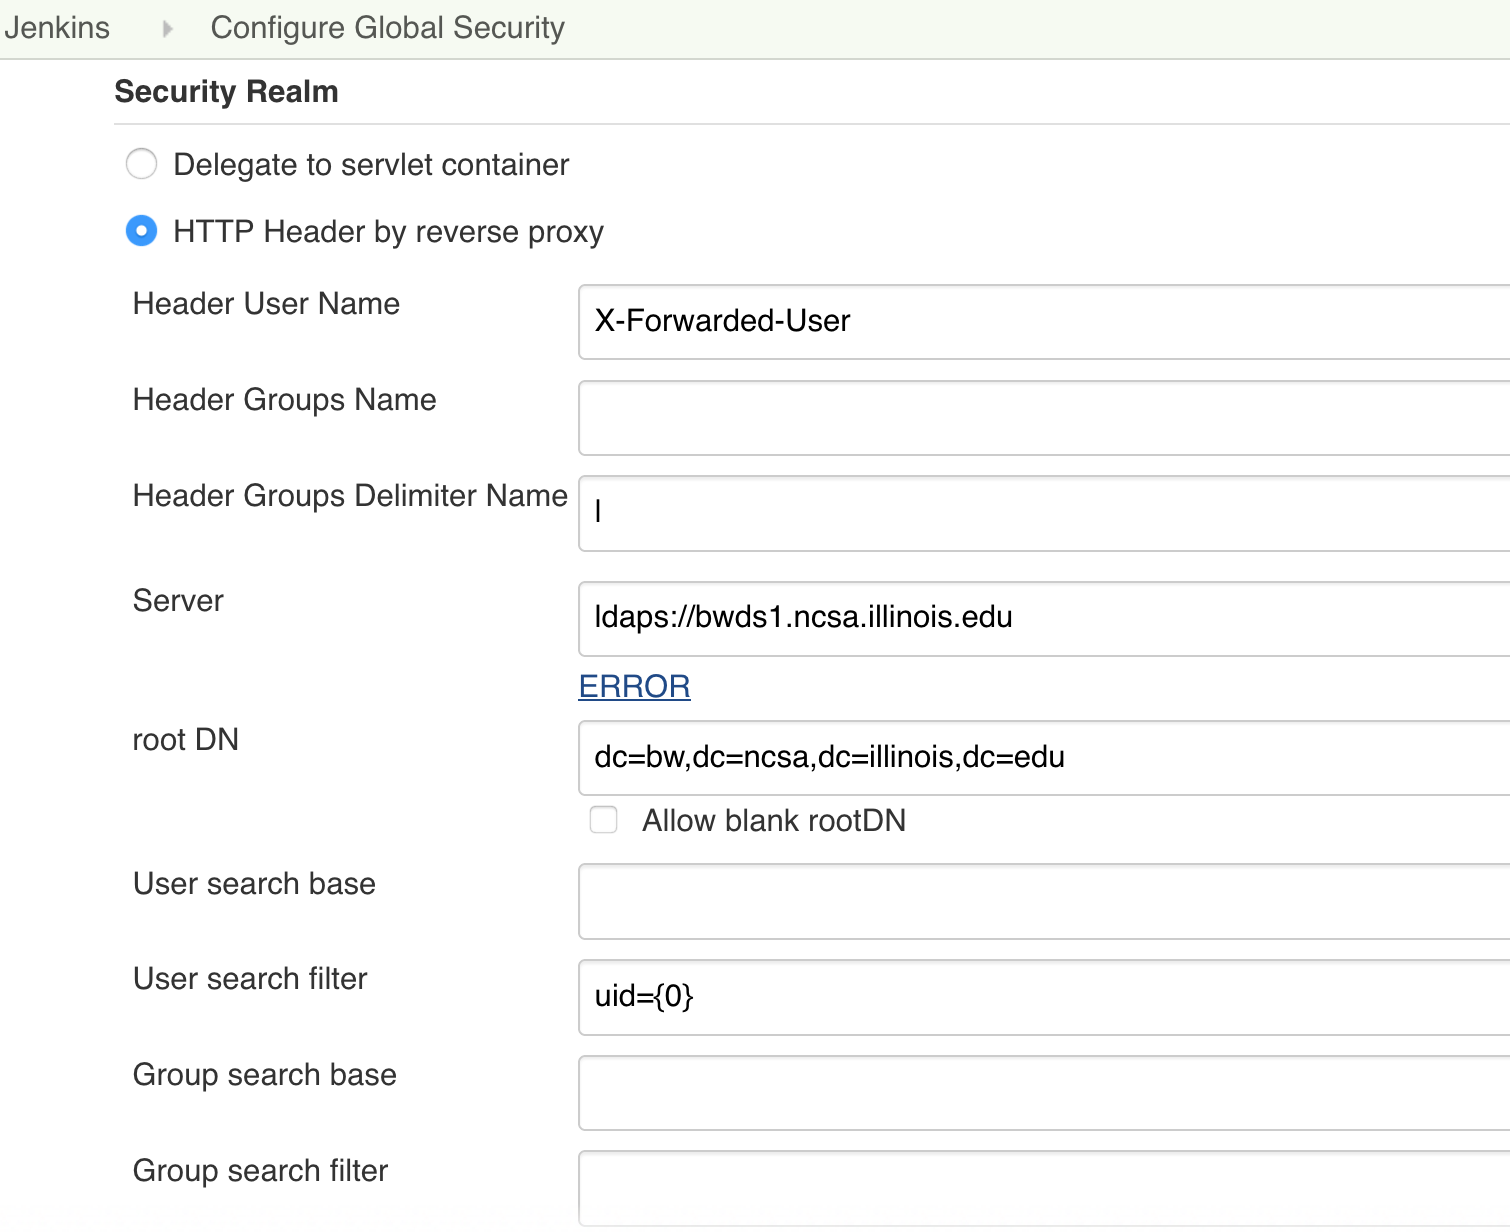
\includegraphics[width=0.5\textwidth]{LDAP-Jenkins}
\caption{ Use LDAP with Jenkins }
\label{fig:LDAP-Jenkins}
\end{figure}
To enable LDAP, the LDAP Plugin was installed. To configure, from the console view, select Manage Jenkins, then select Configure Global Security. In the Security Realm section select the Advanced... tab. Input your LDAP server name and root DN. Click the Test Button.\\
At first this failed because our LDAP is using a local CA.
WARNING: Failed to search LDAP for username, 
sun.security.provider.certpath.SunCertPathBuilderException:
unable to find valid certification path to requested target\\
\\
We had to add our certificate to the keystore:
/usr/java/default/jre/bin/keytool -list -keystore cacerts -imle /etc/openldap/cacerts/cacert.pem
Enter keystore password: Trust this certificate? [no]:  yes\\
Certificate was added to keystore

\subsection{Configure Global Security}
\begin{figure}[H]
\centering
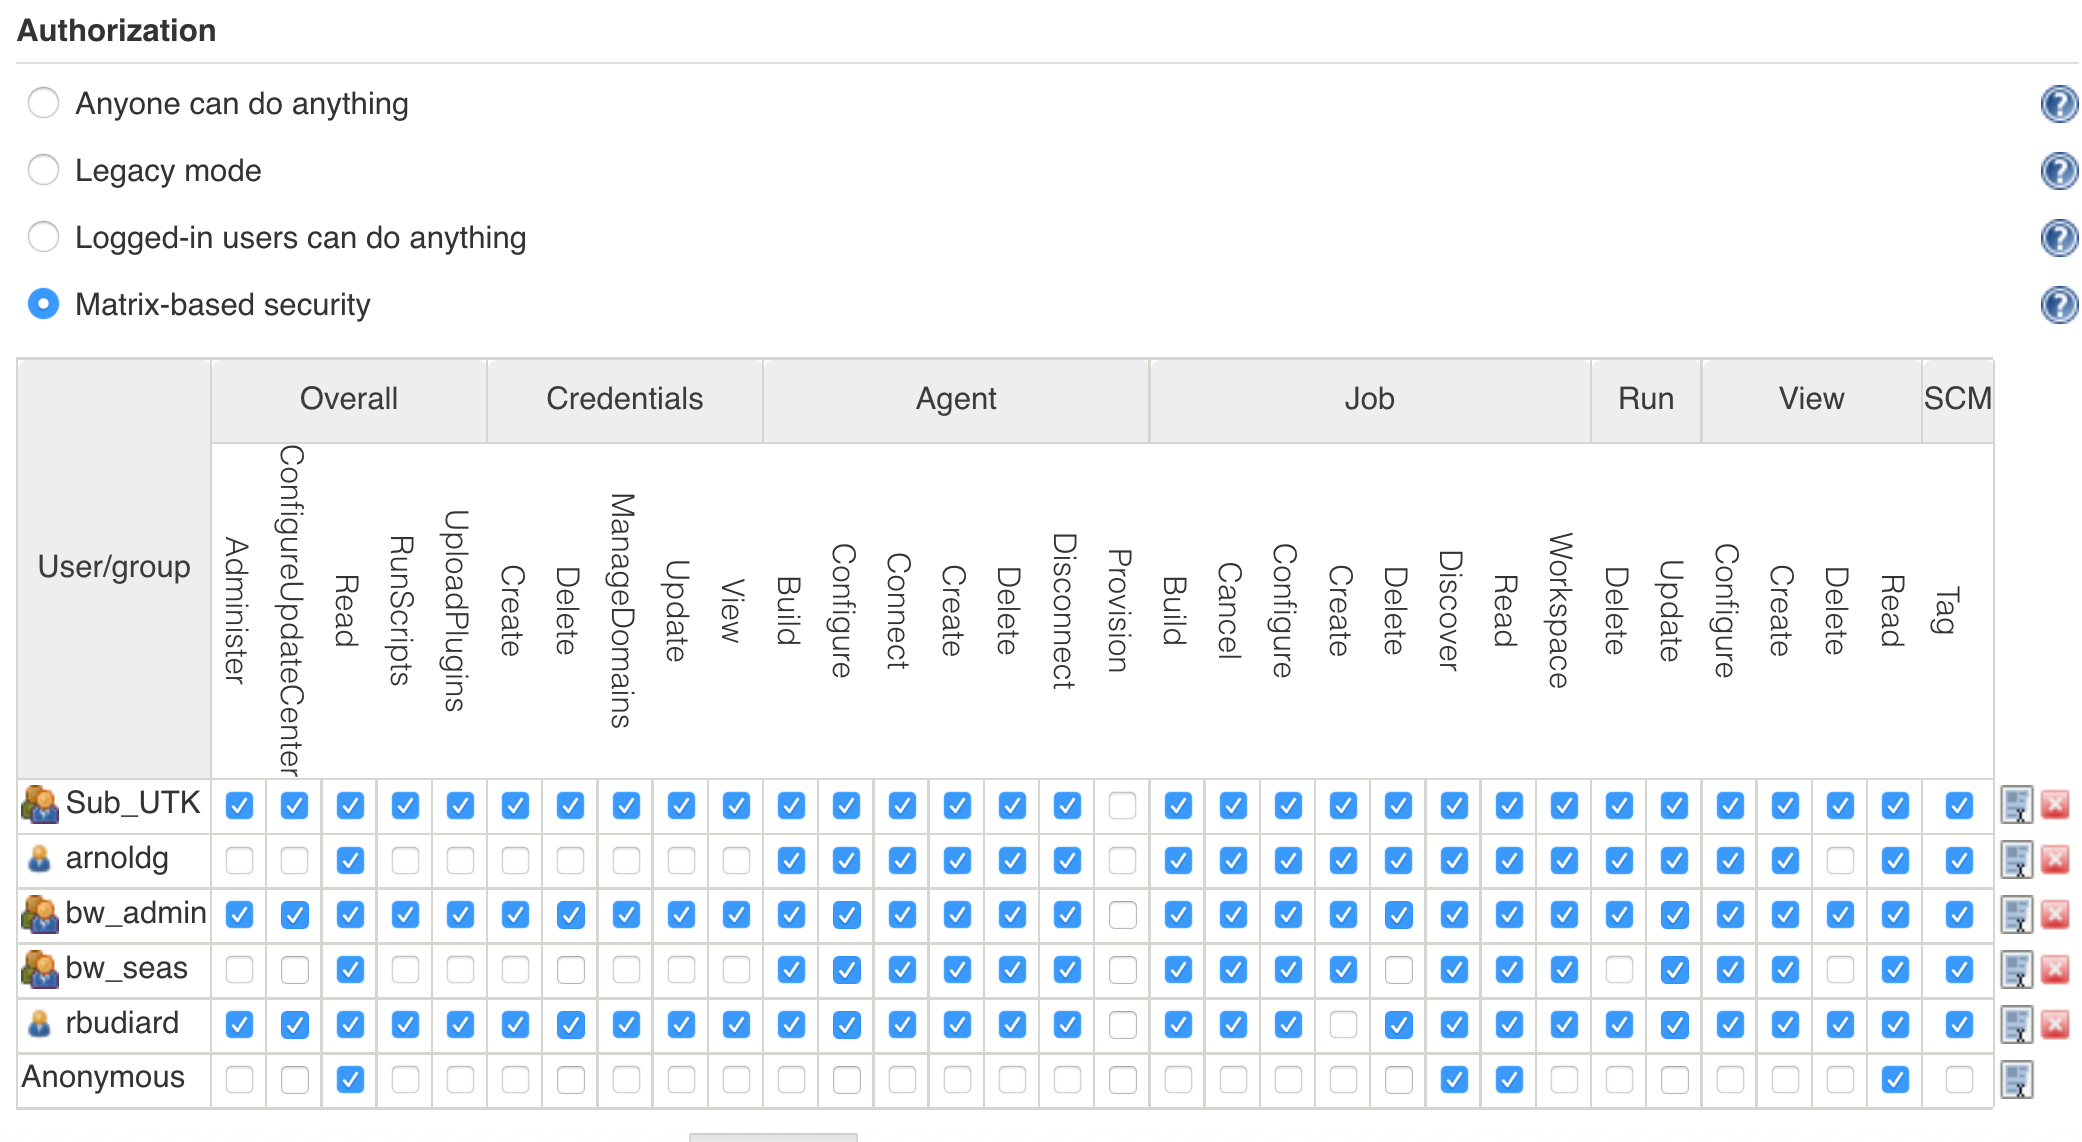
\includegraphics[width=0.5\textwidth]{Configure-Global-Security}
\caption{ Configure Global Security }
\label{fig:Configure-Global-Security}
\end{figure}
We are allowing access by username and LDAP groups. The permissions can be scoped for individuals and groups. An example is removing Job delete permissions to prevent one user or group from deleting each other's jobs. 

\section{Anatomy of A Test}
\label{sec:TestAnatomy}
New software projects are required to be tested on our TDS and approved before deployment on Blue Waters and this is one of our key best practices.  Once a test is deployed it is assigned to a specific Jenkins tab via the "Edit View" link associated with that tab.  Tests still in development reside in the "All" tab view until they have been peer reviewed by at least one other test developer.
\subsection{test description}
We require a description for each test to describe: what is tested, resources used by the test, intent of the test, and scheduling frequency.
\subsection{limits log files}
The Jenkins test VM filled to capacity after the first few weeks of intensive use and an influx of several new tests that output long source code build detail.  We retroactively modified all tests to limit the number of old build logs retained (max 50 for most tests). 
\subsection{ssh to a login host}
There are several target ssh hosts which may be selected from our instance: the test rack JYC, the main system, and the new software deployment login node within the main system.  None of our tests run locally within the Jenkins VM.
\subsection{run shell commands}
A test is composed of shell command and where possible we try to be as transparent with our test construction as possible.  We prefer commands in the Jenkins configuration over running a script in the filesystem on the remote ssh target.  Scripts that are remote run with verbose mode or are displayed via "cat -n" to save output to the Jenkins console log and make for simpler debugging when a test fails.
\subsubsection{test completes on login node}
Some tests run only on the ssh login node and return more or less immediately.  Examples include tests for batch system functionality, ssh functionality, and filesystem functionality.  These tests are very similar in style to unit tests which target a limited set of functionality.
\subsubsection{test is submitted to batch system}
More comprehensive tests typically build and run an application or benchmark through the batch system.  These tests exercise multiple aspects of the system: (filesystem, compilers and modules, high-speed network, external connectivity to the internet...).  They block to completion so that we do not overburden the batch system with tests.  Unlike tests that run entirely on a login node, completion time can be highly variable depending on the queue depth and available backfill windows for the batch system.
\subsection{post test actions}
\subsubsection{scp files back to Jenkins host}
Most comprehensive tests produce output that we use when debugging a failed test.  They may also produce plot data.  These files are copied back to the Jenkins host so that they can be viewed and/or incorporated into the plot feature of Jenkins.
\subsubsection{plots}
Successful tests save plot files and contribute a new data point to a plot.  The Jenkins server accumulates the data as rows in a spreadsheet (under /var/lib/jenkins/jobs/ ) and plots them via the "Plots" link for a test.
\subsection{email notification}
When the state of a test changes, email notification is sent to the test owner.  As a best practice we also use the email notification as a method of tracking authorship and each test has an email owner even if notifications are disabled for the test.


\section{SWTools Integration}
\label{sec:SWToolsIntegration}
\subsection{SWTools with Jenkins}
%\begin{figure}[H]
%\centering
%\includegraphics[width=0.5\textwidth]{swtools-Jenkins}
%\caption{ Use SWTools with Jenkins }
%\label{fig:swtools-jenkins}
%\end{figure}

\subsection{SWTools with Lammps}
\begin{figure}[H]
\centering
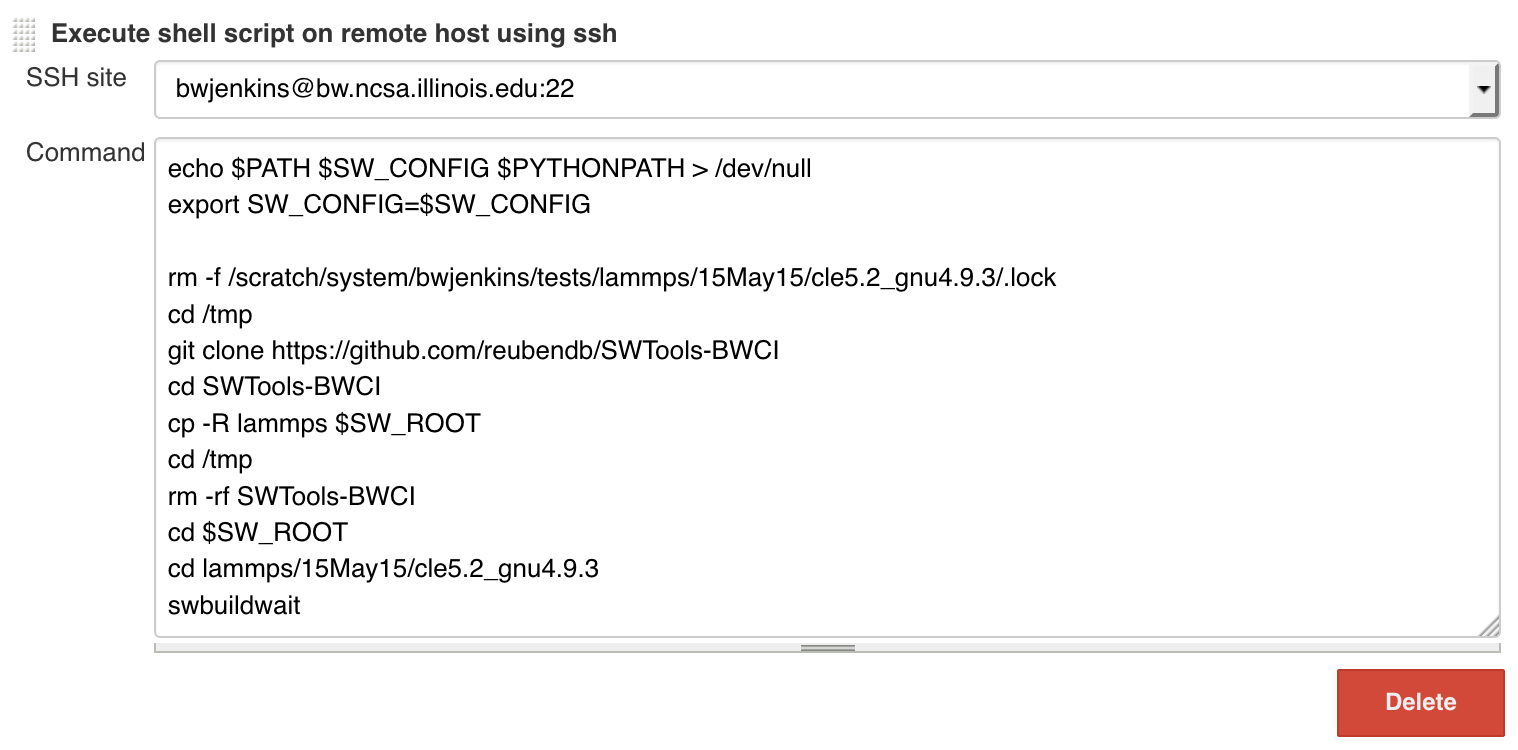
\includegraphics[width=0.5\textwidth]{swtools-lammps}
\caption{ SWTools with Lammps }
\label{fig:swtools-lammps}
\end{figure}

\section{Use Cases}
\label{sec:results}
\subsection{IOR Lustre scratch test}
We created Jenkins tests to periodically run the IOR MPI parallel i/o benchmark at modest scale and validate filesystem functionality and performance for the scratch filesystem. The test is scaled to provide representative performance numbers for a typical small application while not creating performance issues with other jobs or the larger filesystem.  One of our best practices is to provide a management level summary description for casual jenkins users who want to view the tests but do not need to understand the full Jenkins configuration and execution details.  
\begin{figure}[H]
\centering
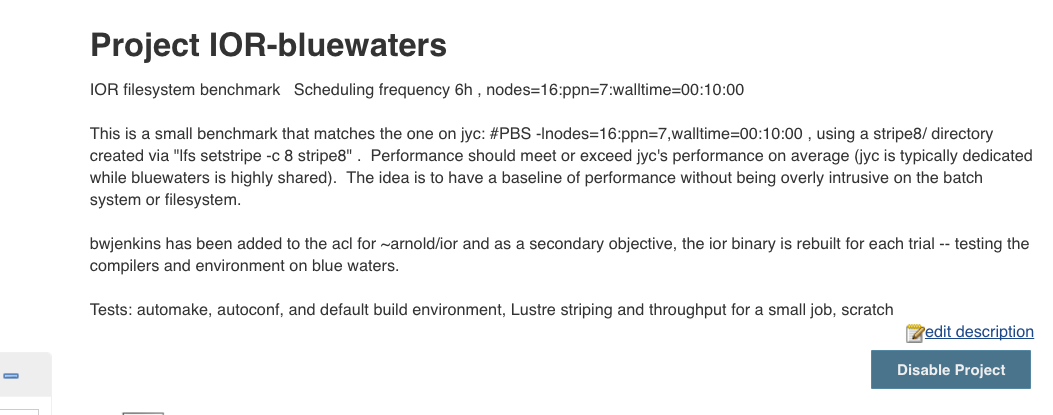
\includegraphics[width=0.5\textwidth]{IOR-bluewaters-descr}
\caption{ IOR description in jenkins }
\label{fig:IOR-bluewaters-descr}
\end{figure}
Where possible, tests build from source and exercise multiple user-facing system components such as: git for external connectivity and modules to test defaults in the environment.  Where scripts on the remote SSH site are used, they are echoed and/or displayed with "cat -n" to make console output verbose and easy to debug in case of errors.  
\begin{figure}[H]
\centering
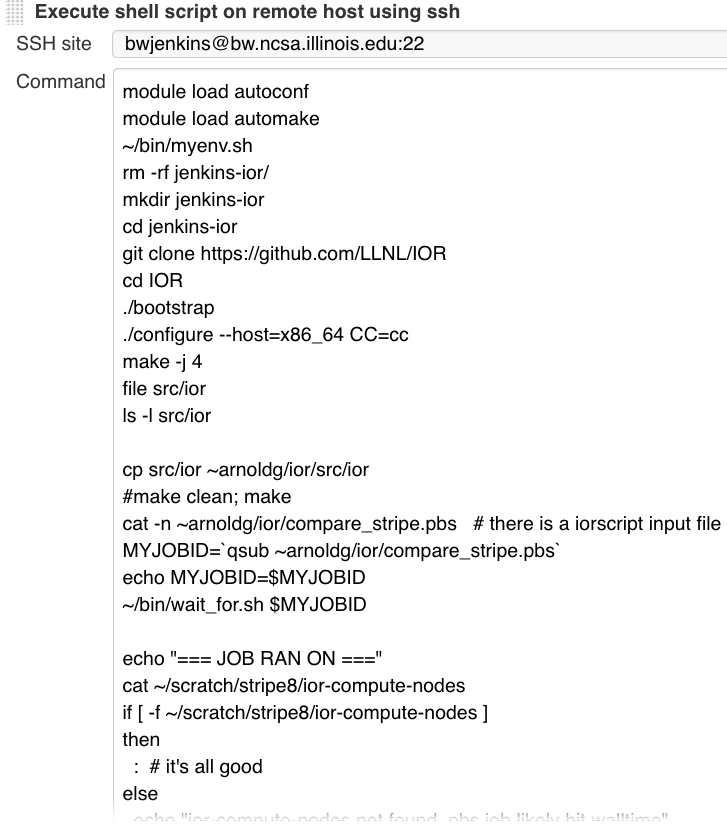
\includegraphics[width=0.5\textwidth]{IOR-configuration-sample}
\caption{ IOR configuration sample }
\label{fig:IOR-configuration-sample}
\end{figure}
The IOR test is set to run as scheduled by Jenkins with a best-effort through our batch system.  The test synchronously blocks such that the next test will not start until the previous one has completed.  We employ a watchdog script to monitor the batch queue and keep the test active until the system marks it as finished.  This has the side effect of making the minimum test time an integer multiple of the sleep time in the watchdog script.  This may be adjusted to fit individual site needs.
\begin{lstlisting}[frame=tb,captionpos=t,language=bash,caption={pbs/torque watchdog script}, label=lst:watchdog]
#!/bin/bash
echo "=== RUNNING $0 ==="
if [ $# -lt 1 ]
then
  echo "$0: missing argument for jobid"
  exit 1
fi
while true
do
	MYQSTAT=`qstat $1`
	if test "$MYQSTAT" = ""
        then
		echo $1 finished
		exit
	else
		DATE=`date`
		echo "$DATE: waiting for $1 to finish"
	fi
	sleep 5m
done
\end{lstlisting}

\begin{figure}[H]
\centering
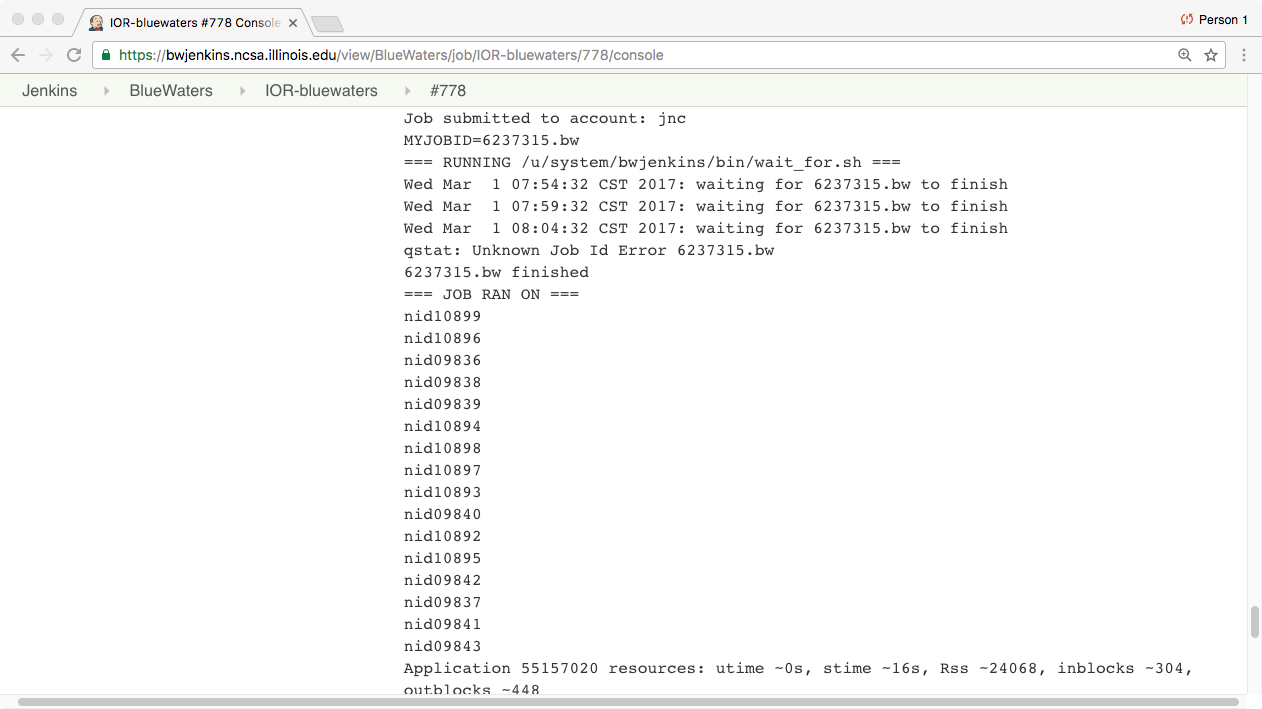
\includegraphics[width=0.5\textwidth]{IOR-watchdog-out}
\caption{ IOR watchdog console output }
\label{fig:IOR-watchdog-out}
\end{figure}
For tests that produce an interesting performance metric like IOR, we save that output to the file format expected by Jenkins and use plotting feature to produce plots. 
\begin{lstlisting}[frame=tb,captionpos=t,language=bash,caption={sample YVALUE output file}, label=lst:yvalue]
bwjenkins$ cat myiorREADnumber.dat 
YVALUE=8352.71
\end{lstlisting}
\begin{figure}[H]
\centering
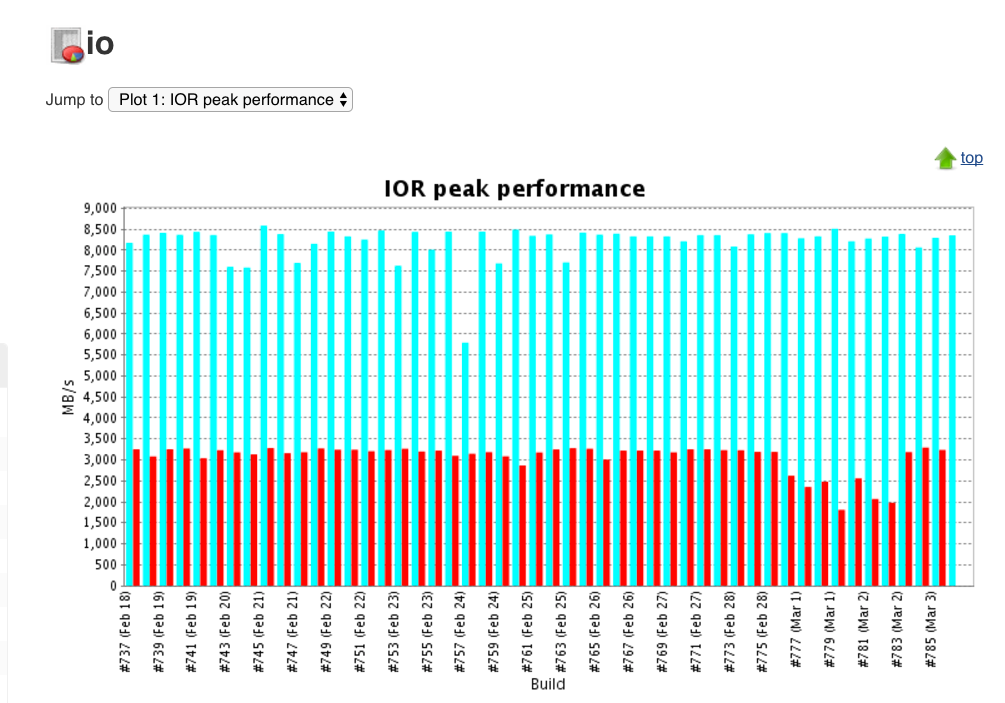
\includegraphics[width=0.5\textwidth]{IOR-plot}
\caption{ IOR plot view }
\label{fig:IOR-plot}
\end{figure}
A plot like this helps us with performance baselines and we can quickly react to changes in the software environment or filesystem configuration that adversely impact performance.

\subsection{mdtest Lustre tests}
The mdtest metadata test is run on the home and scratch filesystems to validate metadata server performance.  The IOR and mdtest user-facing tests complement the fine-grained detail we are able to glean from the backed system-side counters in our OVIS database where we record details about individual server metrics and network traffic on the Cray Gemini fabric.  
\begin{figure}[H]
\centering
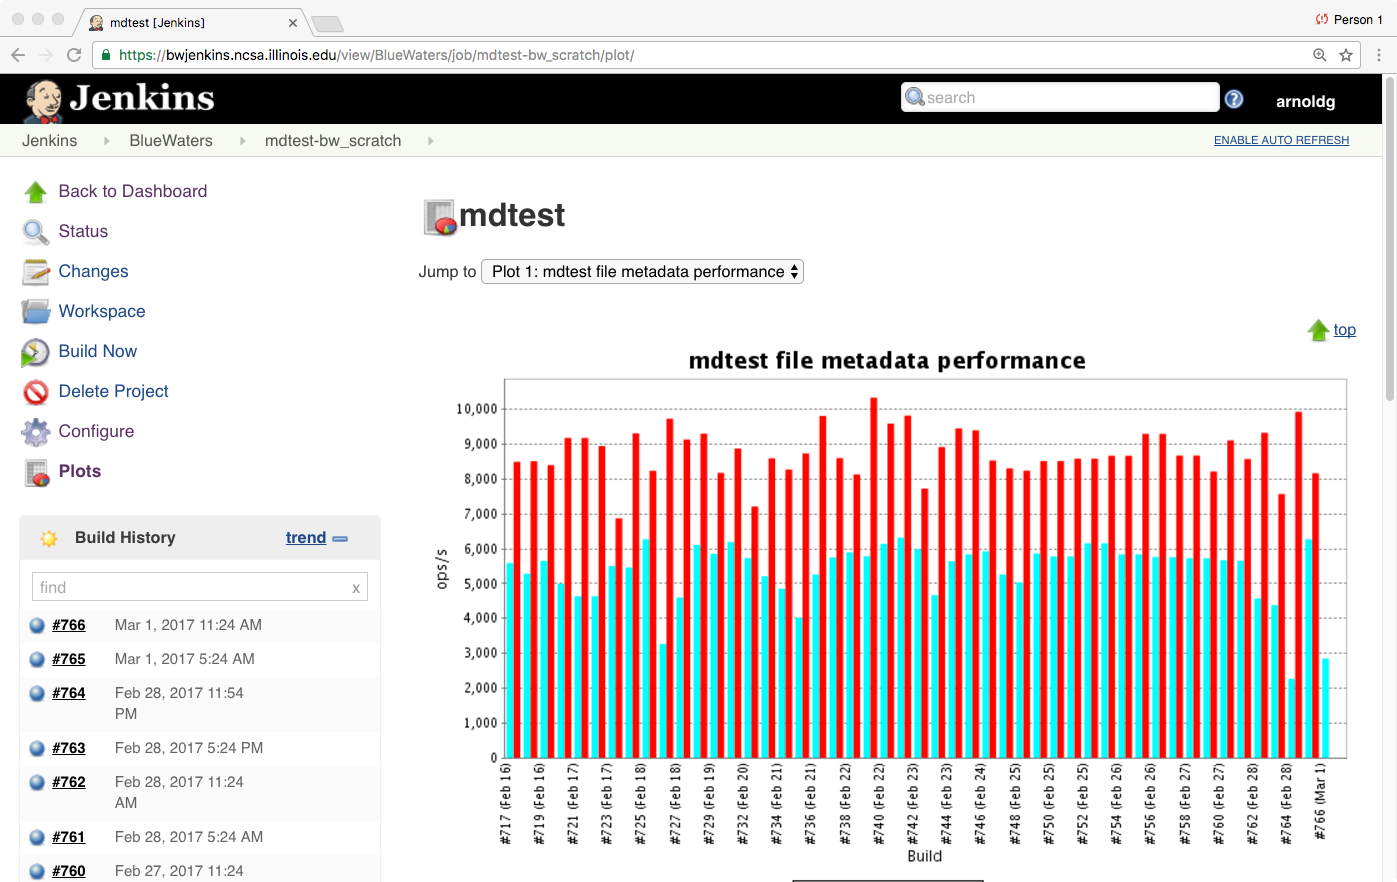
\includegraphics[width=0.5\textwidth]{mdtest-plot}
\caption{ mdtest plot view }
\label{fig:mdtest-plot}
\end{figure}

An additional best practice is to enable E-mail Notifications to the test author and/or other interested parties.  Setting notifications for unstable builds will trigger an E-mail every time the test state changes (from successful to failing and once again when successful ).
\begin{figure}[H]
\centering
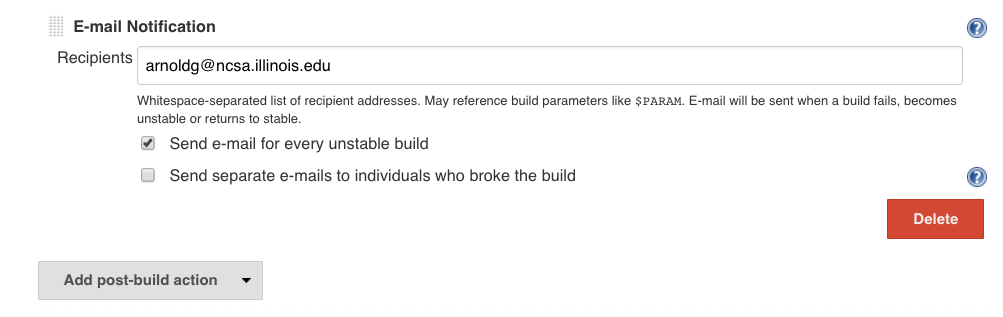
\includegraphics[width=0.5\textwidth]{mdtest-config-email}
\caption{ mdtest email configuration }
\label{fig:mdtest-config-email}
\end{figure}

\subsection{filesystem dashboard}
Our Jenkins instance is a source of information for a filesystem dashboard display we maintain in our wiki.  The "http://" urls for the plot images are shown on the dashboard and provide a recent-time display of filesystem metrics from a user point of view.  We add a Jenkins test to track response time of /bin/ls on the login nodes--a reasonable metric of metadata server health and also the most common problem reported by users when we are having filesystem issues.
\begin{figure}[H]
\centering
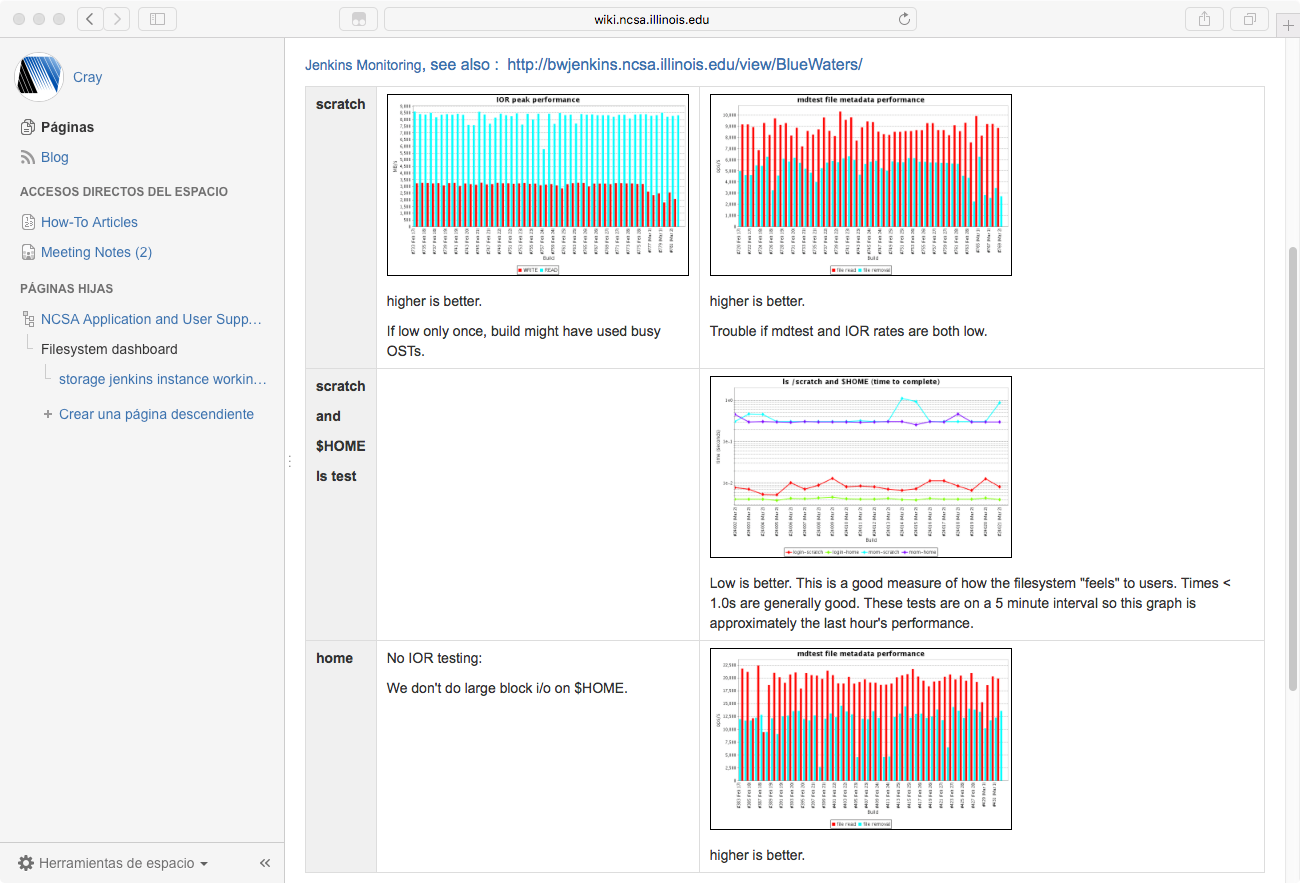
\includegraphics[width=0.5\textwidth]{wiki-dashboard}
\caption{ filesystem dashboard displaying multiple Jenkins plots }
\label{fig:wiki-dashboard}
\end{figure}

\subsection{special projects}
The initial display tabs in our Jenkins instance are used to group tests and we add tabs for special projects.   For example we clone existing tests for evaluating a new software stack on our test login node.   Our test rack has a separate set of tests from our production system and is used as our Jenkins development mule.  The sustained petascale performance benchmarks are in their own tab because they run at scale and are only run on-demand by staff (not scheduled by Jenkins ).
\begin{figure}[H]
\centering
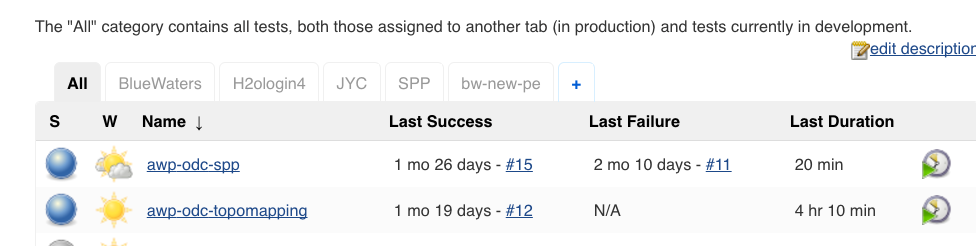
\includegraphics[width=0.5\textwidth]{tabs-display}
\caption{ tabs for project areas }
\label{fig:tabs-display}
\end{figure}

\section{Best Practices}
\begin{itemize}
\item Tests are developed on the JYC development rack and not assigned into a Jenkins tab until reviewed. 
\item Email notification is enabled for most tests and the field is always populated with a test owner.
\item All tests contain a description that describes what is tested, resources required, scheduling frequency, and overall summary  to be readable by the management team.
\item Log file count is limited in the test configuration to keep from filling filesystem space with verbose logs.
\item Tests are coded to be more verbose than necessary so that failures can be isolated quickly and easily.
\end{itemize}

\section{Conclusion}
\subsection{reproducibility and regression testing}
Jenkins provides the framework we need to maintain tests in a consistent fashion and track the results over time (logs and plots ).  Tests typically are not changed so that we get apples-apples comparisons.  When a new test is needed for a particular activity, we attempt to derive it from an existing test to maintain consistency and simplify test creation.  Reusable test components (watchdog scripts, plotting metrics) are employed to make construction of completely new tests straightforward.
\subsection{rapid reaction}
The notification feature keeps test owners engaged in the testing activity of Jenkins and they are often our first responders to system issues.  This results in a shorter reaction time when the system is not performing to expectations--staff are notified automatically when the user experience is impacted.
\subsection{caveats}
\subsubsection{transient errors}
Transient errors with Jenkins sometimes occur--particularly with the Jenkins ssh subsystem.  It's not unusual to get ssh failure rates of 1/100 which are completely transient (immediately running the test again manually clears the issue on the dashboard).
\subsubsection{test scale and frequency}
There is some subjectivity in the frequency and scale (resource utilization) of tests.  Testing too often, too large, or some combination of the two may perturb the system such that other tests are impacted or create bottlenecks in the system for the real user community.  This is the primary reason we require peer review for new tests.
\label{sec:conclusion}

% use section* for acknowledgement
\section*{Acknowledgment}
This research used resources at the National Institute for Computational Sciences (NICS) and the National Center for Supercomputing Applications (NCSA), funded by the National Science Foundation (NSF).

% trigger a \newpage just before the given reference
% number - used to balance the columns on the last page
% adjust value as needed - may need to be readjusted if
% the document is modified later
\IEEEtriggeratref{8}
% The "triggered" command can be changed if desired:
\IEEEtriggercmd{\enlargethispage{-2in}}

% references section
\section*{References}
[1] http://inca.sdsc.edu/ Inca Monitoring: periodic, automated, user-level cyberinfrastructure testing
[2] https://jenkins.io/ Jenkins: open source automation server written in Java

% can use a bibliography generated by BibTeX as a .bbl file
% BibTeX documentation can be easily obtained at:
% http://www.ctan.org/tex-archive/biblio/bibtex/contrib/doc/
% The IEEEtran BibTeX style support page is at:
% http://www.michaelshell.org/tex/ieeetran/bibtex/
%\bibliographystyle{IEEEtran}
% argument is your BibTeX string definitions and bibliography database(s)
%\bibliography{IEEEabrv,../bib/paper}
%
% <OR> manually copy in the resultant .bbl file
% set second argument of \begin to the number of references
% (used to reserve space for the reference number labels box)

%\begin{thebibliography}{9}

%\bibliographystyle{IEEEtran}
%\bibliographystyle{unsrt}
%\bibliography{references}

%\end{thebibliography}

% that's all folks
\end{document}
